\Section{Interface: views}
\label{sec:details}

% This section presents a prototype design of \TI in more details,
% showing preliminary evaluation with promising results.

\Subsection{Network abstractions on demand}
% We first present \Sys's data abstractions. 
The data considered in \Sys is the forwarding plane consisting of all
the switch configurations, \ie FIB.  These ``distributed'' rules
naturally form \Sys \textit{base (stored) tables} and become \Sys's
internal representation of the network forwarding plane. Just like a
distributed network FIB is primarily designed for traffic processing,
the base tables are designed for transaction processing and are not exposed
to \Sys's end users. Externally, \Sys exposes a separate programmable
abstraction called \textit{(network)
  views}.  % Views are customizable,
% users are not confined to any pre-defined sets, user can create and
% destroy views on the fly. 
The customizable view is simply a SQL query which takes base tables as
input, and outputs a new virtual table. A view typically
contains network-wide data, \eg network data selected from nodes
belonging a path or a spanning tree, whichever relevant to a
particular user's task. The view data is also re-structured to simplify
user logic. In the following, we use an example network
(Figure~\ref{fig:eg-one-big-switch}) to illustrate the details.

% to optimize system performance, traffic processing, \eg throughput,
% not for the purpose of managing them from a user (administrator or a
% network application) perspective.
% To extract the data abstraction
% that best suits a user's demand on the fly, \Sys is designed to
% utilize DB view mechanism that allows a user to create abstraction on
% demand.  Specifically, the dataplane is treated as base (\ie stored)
% tables, whereas application data become user views derived from the
% base.
\vspace{-.5em}
\begin{figure}[ht!]
  \centering
  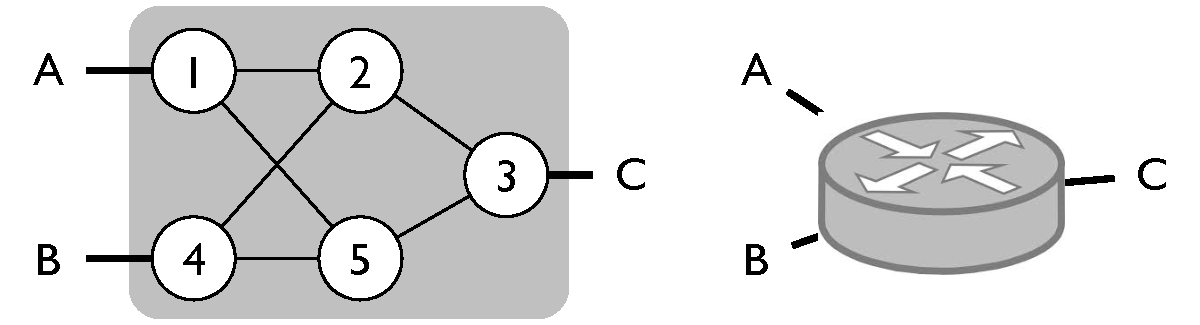
\includegraphics[width=.95\linewidth]{eg-one-big-switch.pdf}
  \caption{\footnotesize Example network and its one big switch
    abstraction}
  \label{fig:eg-one-big-switch}
\end{figure}
\vspace{-1em}

\Paragraph{As base tables} represent a network's
forwarding state, its role is to hide hardware heterogeneity, enable
transaction processing, and ease the creation of external
abstractions. Hence, they hold all the network
(configuration) data in a unified form that is easily accessible.  A
natural choice is a relational model~\cite{hull_relative_1984} that 
consists of three tables: \nd{topology} table that models network as a
pool of resource capacity, \nd{configuration} table that is the union
of all FIBs, and an optional \nd{constraint} table for 
network constraints (\eg SLAs).  \Eg Table~\ref{table:base-table}
shows example table instances.
% annotated topology table~\ref{tb:topology} represents the network's
% resource limit, whereas the flow table
% configuration~\ref{tb:configuration} is a snapshot of the network's
% allocated resource.
All tables are populated when the network is set up (assuming the FIBs
configured pro-actively), and incrementally updated afterwards as
network topology and/or configuration changes.

\begin{table}[ht!]
\begin{subtable}[t]{0.5\linewidth}
  {
    \footnotesize
    \subcaption{topology}
      \begin{tabular}[t!]{c|c|c|c}
        \centering
        node & node & avail\_bw  & used\_bw \\
        \hline
        1 & 2 & 3 & 2 \\
        1 & 5 & 5 & 0 \\
        \multicolumn{4}{c}{...}\\
        \hline
        4 & 5 & 5 & 0 \\
        4 & 2 & 5 & 0 \\ 
        \multicolumn{4}{c}{...}
        \label{tb:topology}
    \end{tabular}
  }
\end{subtable}
\;
\begin{subtable}[t]{0.45\linewidth}
  {
    \footnotesize
    \subcaption{per\_switch configuration}
    \centering
    \begin{tabular}[t]{c|c |c|c}
      \centering
      switch & flow & next & bw \\
      \hline
      1 & 1 & 2 & 1 \\
      1 & 2 & 2 & 1  \\
      \multicolumn{4}{c}{...}\\
      \hline
      2 & 1 & 3 & 1 \\
      \multicolumn{4}{c}{...}\\
      \hline
      3 & 1 & C & 1 \\
      \multicolumn{4}{c}{...}
      \label{tb:configuration}
    \end{tabular}
  }
\end{subtable}
\caption{\footnotesize Example base tables}
\label{table:base-table}
\end{table}
\vspace{-1em}

\Paragraph{The user-defined virtual views} are external
abstractions interfacing with users that are derived from the base tables as SQL
queries and serve as a logical perspective for a user's task. Compared to the
logical contexts introduced in earlier
works~\cite{ethane-sigcomm07,virtual-forwarding-plane}, the strength
of \Sys views is that it does not confine users to preselected
frozen abstractions, instead \Sys views can be created and changed by
users on demand by simply issuing or modifying a SQL query,
which selects from the distributed base tables the relevant
information and restructures them into a network-wide data-structure
that fits the user's task.

\begin{table}[ht!]
  \centering
\begin{subtable}[t]{0.3\linewidth}
    \centering
  {\footnotesize
    \subcaption{routing policy}
      \begin{tabular}[t]{c|c}
        flow & path\_vector \\
        \hline
        1 & (1,2,3) \\
        2 & (1,2,4) \\
        3 & (4,5,3) \\
        \multicolumn{2}{c}{...}
        \label{tb:routing} 
    \end{tabular}
    }
  \end{subtable}
  \;
  \begin{subtable}[t]{0.33\linewidth}
    \centering
  {\footnotesize
    \subcaption{end\_to\_end policy}
    \begin{tabular}[t]{c|c|c}
      flow & ingress & egress \\
      \hline
      1 & 1 & 3 \\
      2 & 1 & 4 \\
      3 & 4 & 3 \\
      \multicolumn{3}{c}{...}
      \label{tb:endpoint}
    \end{tabular}
    }
  \end{subtable}
  \;
  \begin{subtable}[t]{0.3\linewidth}
    \centering
  {\footnotesize
    \subcaption{one\_big\_switch}
    \begin{tabular}[t]{c|c}
        flow & next \\
        \hline
        1 &  C  \\
        2 & B \\
        3 & C \\
        \multicolumn{2}{c}{...}
        \label{tb:rule-capacity}
      \end{tabular}
    }
  \end{subtable}        
  \caption{\footnotesize Example views.}
\label{table:eg-views}
\end{table}

For example, a network-wide routing policy is nothing but the abstract
data as a view (Table~\ref{tb:routing}), derived from the per-switch
\nd{configuration} table, by the following query:
\begin{sql}
CREATE VIEW routing_policy AS (
  SELECT DISTINCT c.flow_id, fp.path_vector
  FROM configuration c 
       NATURAL JOIN flow_policy_fun(c.flow_id) fp
  ORDER BY c.flow_id );  
\end{sql}
In line 2, the \nd{select} statement selects two attributes to from
the view schema: attribute \nd{flow\_id} from \nd{configuration} and
\nd{path\_vector} from \nd{flow\_policy\_fun} which is a recursive
function that computes routing path for \nd{flow\_id}. 
% The \nd{JOIN} statement allows flows to be returned in the absence
% of configuration.  The resulting table of two attributes
% \nd{flow\_id} and \nd{path\_vector} forms the \nd{routing\_policy}
% view.
Similarly, we can derive a one-big-switch configuration view from
\nd{configuration} table and the \nd{obs\_mapping} table which keeps
tracks of the constituting physical nodes \nd{p\_node}.
\begin{sql}
CREATE VIEW obs_configuration AS (
  SELECT flow_id, t.next_id
  FROM   configuration t INNER JOIN obs_mapping ob
  ON     t.switch_id = ob.p_node );  
\end{sql}

Since a view is virtual, only its definition (the query) is stored.
Codd's relational model ensures that a SQL query outputs nothing but tables
(relations), allowing users to use views exactly as a table. A direct
usage is to create views on top of views. The next example shows how to
create an end-to-end policy (Table~\ref{tb:endpoint}) view from
\nd{routing\_policy} view:
\begin{sql}
CREATE VIEW e2e_policy AS (
 SELECT flow_id,
       path_vector[1] AS ingress,
       path_vector[array_length(path_vector,1)] AS egress
 FROM  routing_policy
 ORDER BY flow_id ) ;  
\end{sql}

% OR     t.next_id   = ob.p_node
% For example, \textit{rule capacity} (Table~\ref{table:eg-views}) is
% an example provision view created by the administrator, collecting
% rule capacity information for each switch, endpoint
% (Table~\ref{tb:endpoint}) and routing policy
% (Table~\ref{tb:routing}) are two application views that specify the
% endpoint policy and routing policy respectively.

\Subsection{Network abstraction updates}

A network is in constant change. A virtual view is useful only if its
records are fresh -- reflecting the latest network instantly. For
example, when per-switch rules change, a query on the high-level
policy view \nd{e2e\_routing} (Table~\ref{tb:endpoint}) shall
automatically returns the updated \nd{e2e} reachability. Conversely,
to enable network manipulation via views, the base tables need to be
updated to reflect operations on the views.  For example, to set a new
route \nd{(1,5,4)} for \nd{flow 1} in the example network
(Figure~\ref{fig:eg-one-big-switch} (left)), a user simply insert a new
record denoting the path into the \nd{routing\_policy} view with
\nd{flow} attribute set to \nd{1}. \Sys is responsible of pushing this
abstract view insert into the relevant base \nd{configuration}
inserts.

Generally, view maintenance that keeps virtual views fresh and view
update that synthesizes the base table changes, jointly form a
bi-directional data synchronizer between the base and the view. While
modern DBSes implement view maintenance very efficiently, view update
is supported for restricted
cases~\cite{ak-view-udpate-thesis,relational-lenses}. This is no
surprise, as view update is the harder one: a view contains only partial
information of the base, it is not always possible to locate a unique
base table update~\cite{Bancilhon:view-update-semantics}. To enable
network operations on views, \Sys takes advantage of existing view
maintenance implementation and extends the support of view updates to
network view updates.

\Paragraph{Real-time view maintenance enables network verification.}
\textit{View maintenance} is well supported in modern database systems
(DBS), which \Sys adopts straightforwardly. Specifically, when a view
generated by SQL query program $q$, is queried by a SQL program $p$,
view maintenance translates $p$ on $q$ into queries $p \circ q$ on the
base tables.
% , hence always returning information that is update to the latest
% network state. On the other hand, since views are virtual, This very
% fast re-computation of $p$ keeps the view fresh.  requiring
% re-computation every time it is referred, an alternative is to
% materialize (actually store) the view to accelerate query on the
% views. In this case, view maintenance incrementally updates the
% materialized view table with regard to base table change.
Interestingly, view maintenance offers exactly what is needed in
real-time network verification: by specifying the property of interests
as $p$ over $q$, view maintenance performs check of $p \circ q$ on
network states on the fly. % As shown in \S~\ref{sec:eval},
% checking reachability on a network with more than 10k nodes costs
% less than 10 ms, magnitudes smaller compared to the typically
% per-rule installation or TE operation delay~\cite{b4,ffc}.

\Paragraph{Real-time view update enables network synthesis.}  
Given the ambiguity and non-existence in view update, we first
characterize the correctness criteria in networking. We identify
updates that keep a view's independent and complementary counter-parts
constant. Two views are \textit{independent} if the update on one does
not affect that on the other. Two views are \textit{complementary}, if
they contain enough information to recover the base tables.
% , \ie there alawys exists some base table updates that correctly
% reflect the updated view while keeping the rest views constant.
% In \Sys, it is desirable for views to be independent so they don't
% conflict each other. 
A view updates that keeps the independent views constant eliminates
accident changes made to other existing views; An update that keep a
view's \textit{complementary} constant is a stronger requirement that
does not pollute any possible views (existing and future ones).

\Sys assumes user views are independent, and only performs updates
that keep independent views constant.  In the current prototype, view
update is implemented by hand coded triggers, the call-back functions
that are automatically fired to update the bases when the associated
view update is issued. We evaluate this manual implementation (details
in \S~\ref{sec:eval}) to measure the DB induced delay.
Ultimately, \Sys aims for a generic view update algorithm that
synthesizes for any user-defined views. (We have sketched a novel
algorithm, omitted due to space.) We leave the implementation of the
generic algorithm for future work.

% \input{preliminary-eval}
